\documentclass{article}

\usepackage[english]{babel}
\usepackage[utf8]{inputenc}
\usepackage{amsmath}
\usepackage{graphicx}
\usepackage[breaklinks]{hyperref}
\usepackage[font=footnotesize,labelfont=bf,margin=2.5cm]{caption}
\usepackage{listings}
\usepackage{subfigure}
\usepackage[round]{natbib}
\bibliographystyle{plainnat}


\title{
	Project 02 \\
	\bigskip
	\normalsize APSC 607 Fall 2017
}

\author{Seth Goodman}

\date{\today}


\begin{document}
\maketitle


%\begin{abstract}
%\end{abstract}

\section{Introduction}
\label{sec:introduction}

This project explores different numerical methods for calculating the definite integrals of functions. Two functions will be examined in the range between zero and two, using the Composite Trapezoidal Rule, Composite Midpoint Rule, and Composite Simpson’s Rule, as well as an adaptive implementation of Simpson’s Rule. The behavior and characteristics of these methods will be reviewed and their accuracy evaluated at varying number of subintervals, \textbf{n}. For each \textbf{n}, the result will be compared to the true integral value, using tolerance thresholds to determine sufficient levels of accuracy. 
  		  
All computations are performed using MATLAB using the code accompanying this report. Section \ref{sec:methods} will present the methods used in MATLAB to explore functions. Section \ref{sec:results} contains the results and related outputs for each function along with observations and discussion. All figures and tables found in this report are available in the output subdirectory of the accompanying zip file. Additionally, all code and figures found in the zip file can be accessed via GitHub\footnote{\url{https://github.com/sgoodm/apsc607/tree/master/project_02}}

\newpage
\section{Methods}
\label{sec:methods}

The two unique functions which will be explored in this project, Functions \textbf{A} and \textbf{B}, are defined by Equations \ref{eq:fa} and \ref{eq:fb}, respectively.

\begin{center}
    \centering
    \begin{minipage}{0.5\textwidth}
        \centering
        \begin{equation}
		f(x) = e^{2x} * sin(3x)
		\label{eq:fa}
		\end{equation}
    \end{minipage}\hfill
    \begin{minipage}{0.5\textwidth}
        \centering
        \begin{equation}
		f(x) = \frac{1}{x+4}
		\label{eq:fb}
		\end{equation}
    \end{minipage}
\end{center}


To establish a baseline for error comparisons, the true value of the integral of each function is first calculated using built in MATLAB tools. The integral is calculated both using the symbolic toolkit function \textbf{int} as well as the numerical function \textbf{integral}. The resulting values can be seen in Table \ref{true_values}.

\bgroup
\def\arraystretch{1.5}
\begin{center}
	\centering
	\begin{tabular}{l|r|r}
	\textbf{Function} & \textbf{Symbolic} & \textbf{Numeric} \\
	\hline
	A & -14.2139771298625 & -14.2139771298625\\
	B & 0.405465108108164 & 0.405465108108164
	\end{tabular}
	\captionof{table}{True values of integrals between zero and two}
	\label{true_values}
\end{center}
\egroup

The true values for Functions A and B are compared to the results of integration using the Trapezoidal, Midpoint, and Simpson's Rules for a range of subintervals. The range of subinterval values, \textbf{n}, can vary depending on the function and rule tested, in order to ensure that an accuracy within a tolerance of $10^{-4}$ and $10^{-8}$ of the true value is achieved by at least one \textbf{n} value in the range. 

\begin{equation}
error = abs\Bigg[\Big[ \int_{a}^{b}f(x)dx \Big]_{true} - \Big[ \int_{a}^{b}f(x)dx \Big]_{numeric}\Bigg]
\label{eq:tolerance}
\end{equation}

The tolerance is based on the error for a given rule, defined in Equation \ref{eq:tolerance} as the absolute difference between the result of numerical integration at a given \textbf{n} value and the true value of the integral. An alternative approach for measuring tolerance is to compare the difference between the integral resulting from subsequent values of \textbf{n}. Both methods will effectively illustrate the performance of the different methods of numerical integration, but comparing to the true value provides a independent metric of accuracy, rather than one which is dependent on the step size between values of \textbf{n}. Since the accuracy tolerance will not be based on subsequent values of \textbf{n}, a sample of values for \textbf{n} can be used rather than the full range. This drastically improves the performance of the MATLAB calculations in cases where a large range of \textbf{n} needs to be tested, without sacrificing noticeable detail from the results. 

The value of \textbf{n} required to reach the specified tolerance is dependent on the function itself as well as the error term associated with each rule. The error terms for the Composite Trapezoidal, Midpoint, and Simpson's Rules are defined in Equations \ref{trap_err}, \ref{mid_err}, and \ref{sim_err} respectively \citep{burden2010}. As the Trapezoidal and Midpoint Rules have second order error terms, it is expected that they will require a greater value of \textbf{n} to produce results comparable to Simpson's Rule, which has a fourth order error term.

 
\begin{center}
    \centering
    \begin{minipage}{0.3\textwidth}
        \centering
        \begin{equation}
		\frac{b-a}{6}h^2f^{''}(u)
		\label{trap_err}
		\end{equation}
    \end{minipage}\hfill
    \begin{minipage}{0.3\textwidth}
        \centering
        \begin{equation}
		\frac{b-a}{12}h^2f^{''}(u)
		\label{mid_err}
		\end{equation}
    \end{minipage}
    \begin{minipage}{0.3\textwidth}
        \centering
        \begin{equation}
		\frac{h^5}{90}f^{(4)}(\xi_j)
		\label{sim_err}
		\end{equation}
    \end{minipage}
\end{center}

\bigskip


All values of \textbf{n} tested will be positive and even, as it is required for the Midpoint and Simpson's Rules. Although the Trapezoidal Rule can be used with odd intervals, using only even intervals will provide sufficient sample points for analysis. For most cases, the values of \textbf{n} range from 2 to 3000, at intervals of 2. However, in certain cases where it takes roughly 100,000 subintervals to reach the lowest tolerance with the Trapezoidal or Midpoint Rules, a binary expansion is used to generate values of \textbf{n} at which to sample the full range, rather than testing at every possible step. Starting with two sub intervals ($n=2$), if every even sub interval value up to 100,000 was tested it would require 50,000 points. By incorporating a binary expansion based approach in this scenario, a sample of only 20 different \textbf{n} values is generated which are capable of sufficiently demonstrating the behavior of the integration rules\footnote{A larger sample would have been practical, but after the initial implementation of binary based sampling the results were sufficient to demonstrate the overall behavior so there was no reason to modify it further}.


\begin{center}
	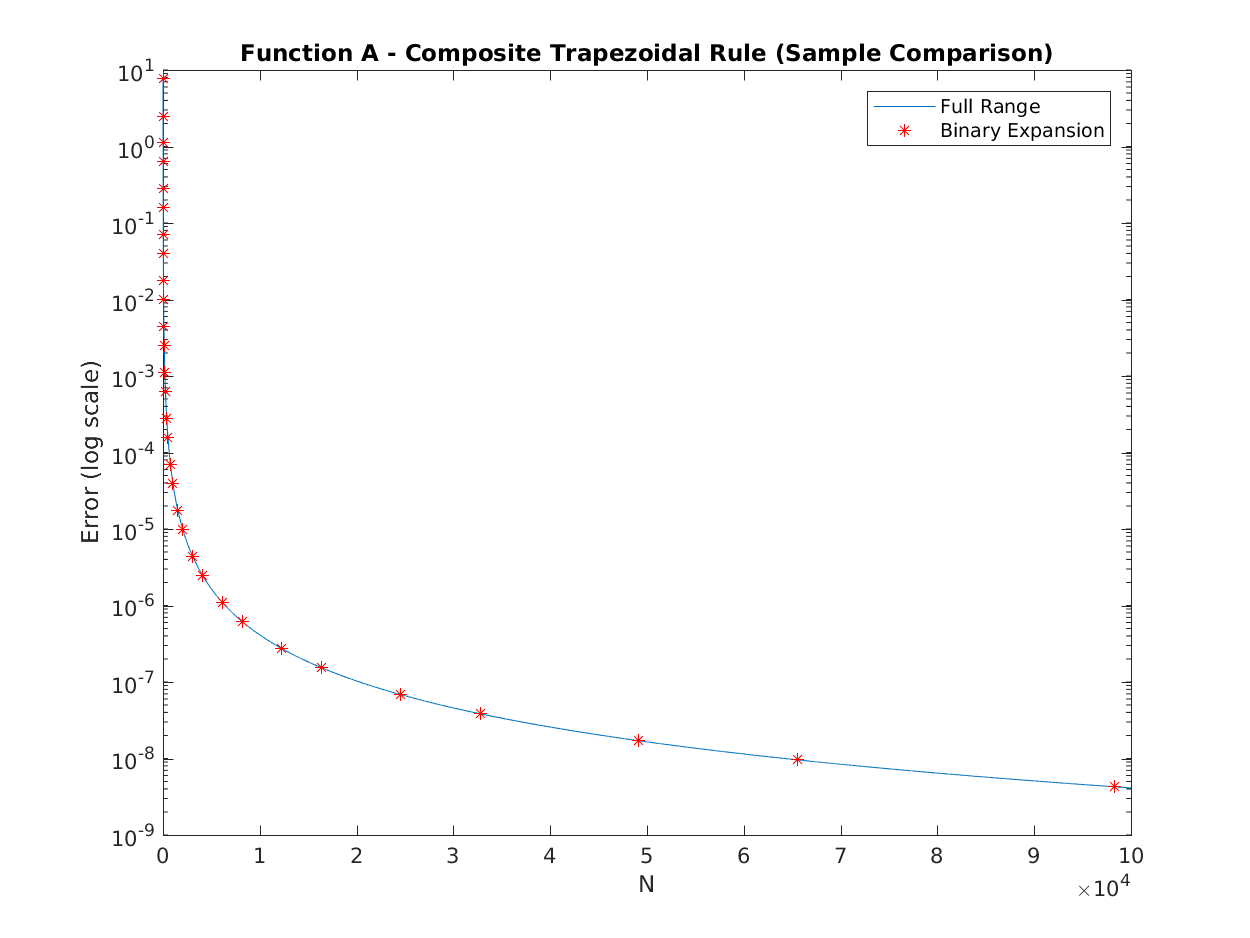
\includegraphics[width=0.75\textwidth]{../output/a_trapezoidal_sample_comparison.png}
	\captionof{figure}{Sample Comparison}
	\label{fig:sample_comparison}
\end{center}

Figure \ref{fig:sample_comparison} illustrates an example of the sampling points used for \textbf{n} ranging between 2 and 100,000. As a tradeoff for reduced computation time, the apparent value of \textbf{n} required to achieve a given tolerance can be inflated as seen in Table \ref{table:sample_comparison}. Sampling may not be ideal in all scenarios, but works well as an exploratory technique when the magnitude of the upper limit of the \textbf{n} values is unknown and/or the potential number of \textbf{n} values which need to be tested is very large.

\bgroup
\def\arraystretch{1.5}
\begin{center}
	\centering
	\begin{tabular}{l|r|r}
	\textbf{Tolerance} & \textbf{Full Range} & \textbf{Sample} \\
	\hline
	$10^{-4}$ & 644 & 768\\
	$10^{-8}$ & 64230 & 65536
	\end{tabular}
	\captionof{table}{Example \textbf{n} needed to reach tolerance by sampling \textbf{n} vs using full range}
	\label{table:sample_comparison}
\end{center}
\egroup


The functions implementing the Trapezoidal, Midpoint, and Simpson's Rules will be called over the range of values for \textbf{n} using the \textbf{arrayfun} function in MATLAB. This function accepts another function, defining our integration rule, and a vector, and simply repeatedly calls the specified value while iterating over the values in the vector. The call to \textbf{arrayfun} then returns a vector (or set of vectors in this case) containing the results from each call to the integration function. A simplified example below show the \textbf{arrayfun} function being used to pass each \textbf{n} value in a vector called \textbf{nlist} to a trapezoidal function, returning a vector of the resulting output values.

\bigskip
\begin{lstlisting}[language=Matlab]
[int_vals] = arrayfun(@(n) trapezoidal(n), nlist);
\end{lstlisting}
\bigskip

The resulting vector of integral values across varying \textbf{n} can compared with the true integral value generated earlier, to produce an error vector. The error vector is used to identify the value of \textbf{n} (and thus \textbf{h}) at which the integration rule produced results that were accurate within a desired tolerance. No \textbf{n} value needs to be specified for the adaptive approach because, as seen in Subsection \ref{method:adaptive}, this approach iteratively checks (within the function) that a specified tolerance has been reached before producing a single output rather than using a set \textbf{n} value to produce a set of output values.

The remainder of this section will introduce the three composite numerical integration approaches (Trapezoidal, Midpoint, and Simpson's) and the adaptive approach using Simpson's Rule.


\subsection{Composite Trapezoidal Rule}\label{method:trapezoidal}

\begin{center}
	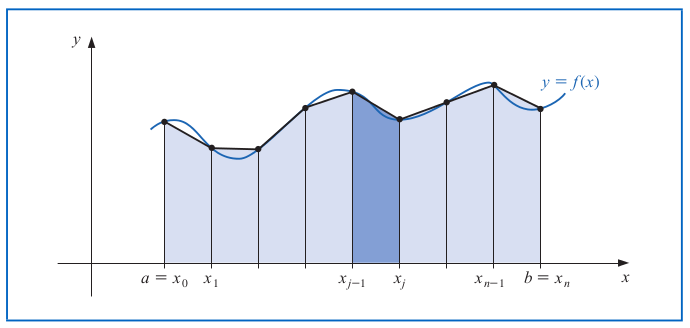
\includegraphics[width=0.9\textwidth]{../additional/trapezoidal_fig.png}
	\captionof{figure}{Trapezoidal Figure \citep{burden2010}}
	\label{trap_fig}
\end{center}


The Composite Trapezoidal Rule for $n$ intervals, as seen in Figure \ref{trap_fig}, can be defined by Equation \ref{trap_eq}, given $h=(b-a)/n$ and $x_j=a+jh$, for each $j=0,1,\dots,n$ \citep{burden2010}.

\begin{equation}
\int_{a}^b f(x) dx = \frac{h}{2} \Bigg[ f(a) + 2 \sum_{j=1}^{n-1} f(x_j) + f(b) \Bigg]
\label{trap_eq}
\end{equation}

In this equation, the integral of each individual subinterval is calculated simply as the area of a trapezoid:

\begin{equation}
area_{subinterval} = \frac{f(x_j) + f(x_{j+1})}{2}h
\end{equation}


\subsection{Composite Midpoint Rule}\label{method:midpoint}

\begin{center}
	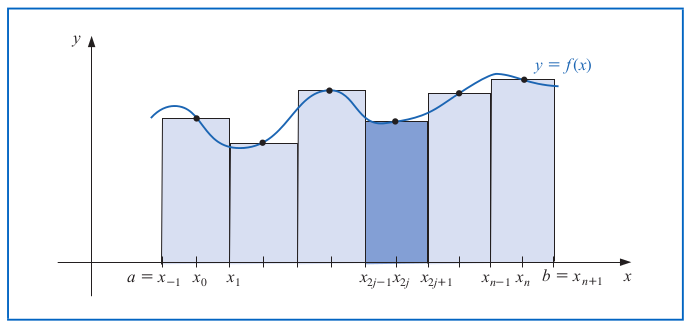
\includegraphics[width=0.9\textwidth]{../additional/midpoint_fig.png}
	\captionof{figure}{Midpoint Figure \citep{burden2010}}
	\label{mid_fig}
\end{center}

The Composite Midpoint Rule for $n+2$ intervals, as seen in Figure \ref{mid_fig}, can be defined by Equation \ref{mid_eq}, given $h=(b-a)/(n+2)$ and $x_j=a+(j+1)h$, for each $j=-1,0,\dots,n+1$ \citep{burden2010}.

\begin{equation}
\int_{a}^b f(x) dx = 2h \sum_{j=0}^{n/2}f(x_2j)
\label{mid_eq}
\end{equation}

The area for each subinterval is similar to the Trapezoidal Rule, but instead of calculated the area of a trapezoid, the midpoint of the subinterval is used to calculate the area of a rectangle:

\begin{equation}
area_{subinterval} = f(\frac{x_{2j-1}+x_{2j+1}}{2})h
\end{equation}

\subsection{Composite Simpson's Rule}\label{method:simpsons}

Unlike the Trapezoidal or Midpoint Rules, Simpson's Rule utilizes subintervals with three points, seen in Figure \ref{sim_fig}, resulting in a higher order error term as seen earlier in \ref{sim_err}.

\begin{center}
	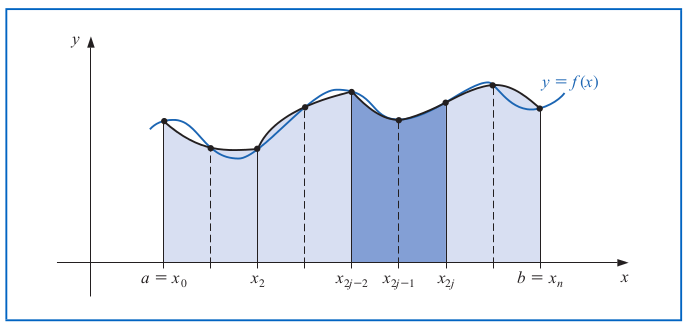
\includegraphics[width=0.9\textwidth]{../additional/simpsons_fig.png}
	\captionof{figure}{Simpson's Figure \citep{burden2010}}
	\label{sim_fig}
\end{center}

The Composite Simpson's Rule for $n$ intervals, as seen in Figure \ref{sim_fig}, can be defined by Equation \ref{sim_eq}, given $h=(b-a)/n$ and $x0_j=a+jh$, $x1_j=a+jh+h/2$, $x2_j=a+jh+h$,  for each $j=0,1,\dots,n-1$.
     
\begin{equation}
\int_{a}^b f(x) dx = \frac{h}{3}\Bigg[ f(a) + 2\sum_{j=1}^{(n/2)-1} f(x_{2j}) + 4\sum_{j=1}^{n/2} f(x_{2j-1}) + f(b) \Bigg]
\label{sim_eq}
\end{equation}



\subsection{Adaptive Simpson's Rule}\label{method:adaptive}

An adaptive integration approach iteratively compares each subinterval (starting with the full range) with the next level of subintervals (splitting the current subinterval in half) until a specified tolerance value (difference between integration value of original subinterval and the sum of the integration of the subinterval halves) has been reached. This process can be modified to calculate integrals using any method, though Simpson's Rule is used through this project. A rough overview of this process is demonstrated using the following pseudocode.

\bigskip
\small
\begin{lstlisting}[language=Python]
# ------------------------------------------------------------
integral_value = 0
subinterval_data = [{
  'a': bound_min, 
  'b': bound_max, 
  'h': (bound_max-bound_min)/2, 
    ...
}]
number_of_subintervals_remaining = 1

while number_of_subintervals_remaining > 0:
  i = number_of_subintervals_remaining
  a, b, h, ... = subinterval_data[i]

  active_integral = simpsons(a,b)

  left_half_integral = simpsons(a, (b-a)/2)
  right_half_integral = simpsons((b-a)/2, b)
	
  number_of_subintervals_remaining -= 1
  
  halves_sum = left_half_integral + right_half_integral
  diff = active_integral - halves_sum 
  	
  if diff < tolerance:    # tolerance reached
    integral_value += active_interval
		
  else:    # tolerance not reached, split in half
    subinterval_data.append(
      {'a': a, 'b': (b-a)/2, 'h': h/2, ... }, # new left half
      {'a': (b-a)/2, 'b': b, 'h': h/2,  ...} # new right half
    )
    number_of_subintervals_remaining += 2
# ------------------------------------------------------------
\end{lstlisting}
\bigskip
\normalsize


\newpage
\section{Results}
\label{sec:results}

This section will review the results of the different integration rules for Functions A and B. An overview of these results can be seen in Table \ref{table:results}, which shows the the number of subintervals required to reach each tolerance specified, as well as the final error achieved. Figure \ref{fig:true} contains the true plots of both function, for reference.

\bgroup
\footnotesize
\def\arraystretch{1.5}
\begin{center}
	\centering
	\begin{tabular}{l|l|r|r|r}
	\textbf{Function} & \textbf{Method} & \textbf{N: $10^{-4}$} & \textbf{N: $10^{-8}$} &\textbf{Minimum Error} \\
	\hline  
	a & trapezoidal & 768  & 65536 & 4.26887e-09 \\
    a & midpoint    & 1024 & 98304 & 8.53747e-09 \\
    a & simpsons    & 42   & 322   & 1.30384e-12 \\
    a & adaptive    & 24   & 278   & -           \\
    b & trapezoidal & 12   & 1082  & 1.29289e-09 \\
    b & midpoint    & 22   & 1522  & 2.58233e-09 \\
    b & simpsons    & 2    & 22    & 2.22044e-16 \\
    b & adaptive    & 2    & 16    & -  
	\end{tabular}
	\captionof{table}{Results}
	\label{table:results}
\end{center}
\egroup

 
\begin{center}
    \centering
    \begin{minipage}{0.5\textwidth}
        \centering
        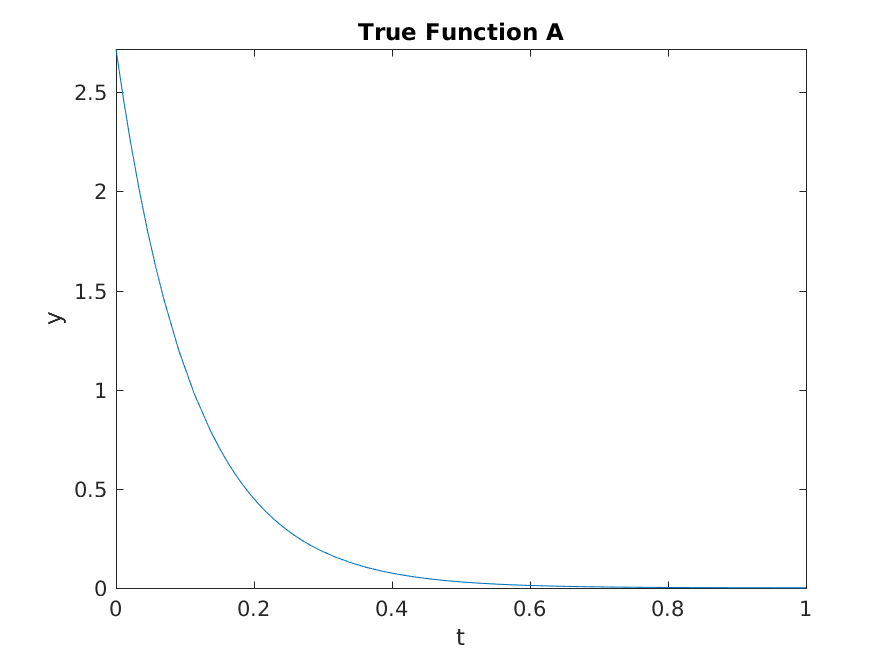
\includegraphics[width=0.99\textwidth]{../output/a_actual.png}
    \end{minipage}\hfill
    \begin{minipage}{0.5\textwidth}
        \centering
        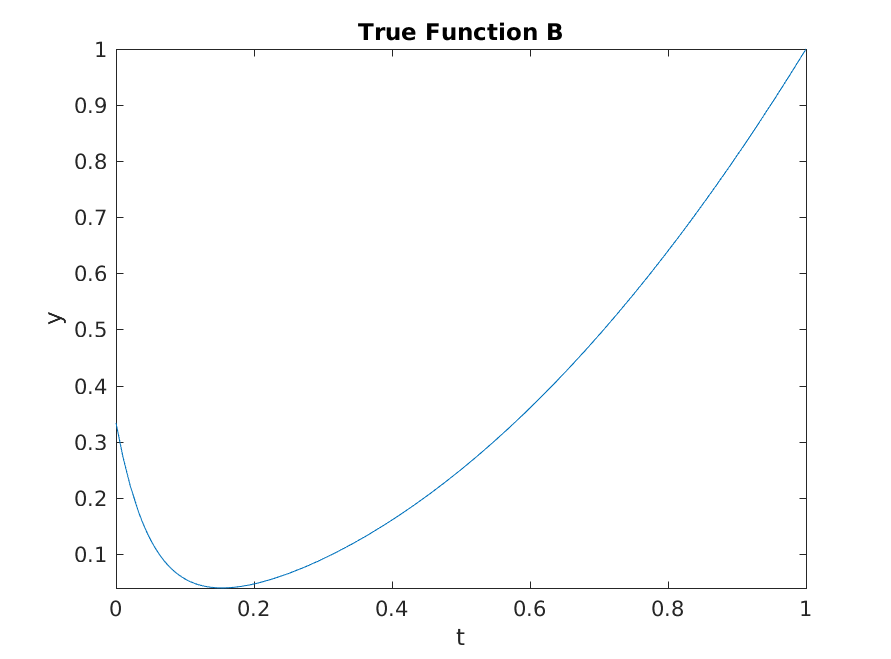
\includegraphics[width=0.99\textwidth]{../output/b_actual.png}
    \end{minipage}
  	\captionof{figure}{True plots of Function A and B between zero and two}
	\label{fig:true}

\end{center}



\subsection{Trapezoidal and Midpoint Results}\label{results:a}

The Composite Trapezoidal and Midpoint Rules performed comparably well to one another, as expected given their similarity - both conceptually and in terms of the equations used to implement them (and the associated error terms) The error plots for the functions using these rules can be seen in Figures \ref{fig:a_trap_mid} and \ref{fig:b_trap_mid}.

Function A require relatively large values of \textbf{n}, nearly 100,000 to reach the lower level tolerance of $10^{-8}$ and necessitated the use of the binary expansion sampling discussed in Section \ref{sec:methods} earlier. Ultimately, the Trapezoidal and Midpoint Rules required an \textbf{n} values of 65,000 and 98,000, respectively, to achieve this tolerance level (seen in Table \ref{table:results}\footnote{As mentioned in the \textit{Methods} section, the values of \textbf{n} listed in Table \ref{table:results} for the Trapezoidal and Midpoint Rules used with Function A are slightly greater than what is actually required to reach the specified tolerance, due to the binary sampling.}.  

\begin{center}
	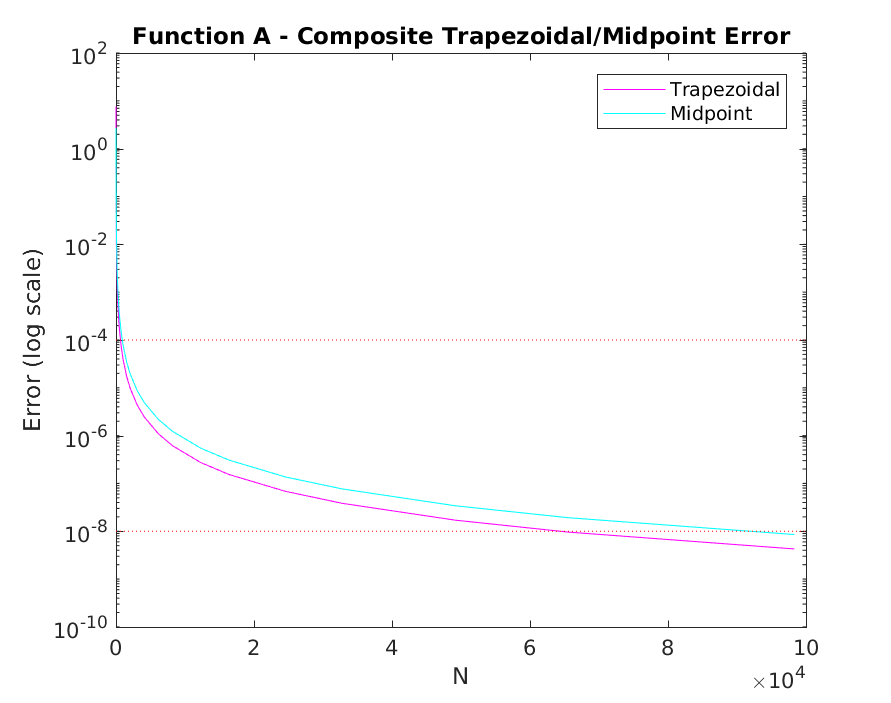
\includegraphics[width=0.7\textwidth]{../output/a_trapezoidal_midpoint.png}
	\captionof{figure}{Plot of error from Trapezoidal and Midpoint integration of Function A}
	\label{fig:a_trap_mid}
\end{center}

The value of \textbf{n} required to reach a tolerance of $10^{-8}$ for Function B was only 1082 and 1522 for the Trapezoidal and Midpoint Rules, respectively.

\begin{center}
	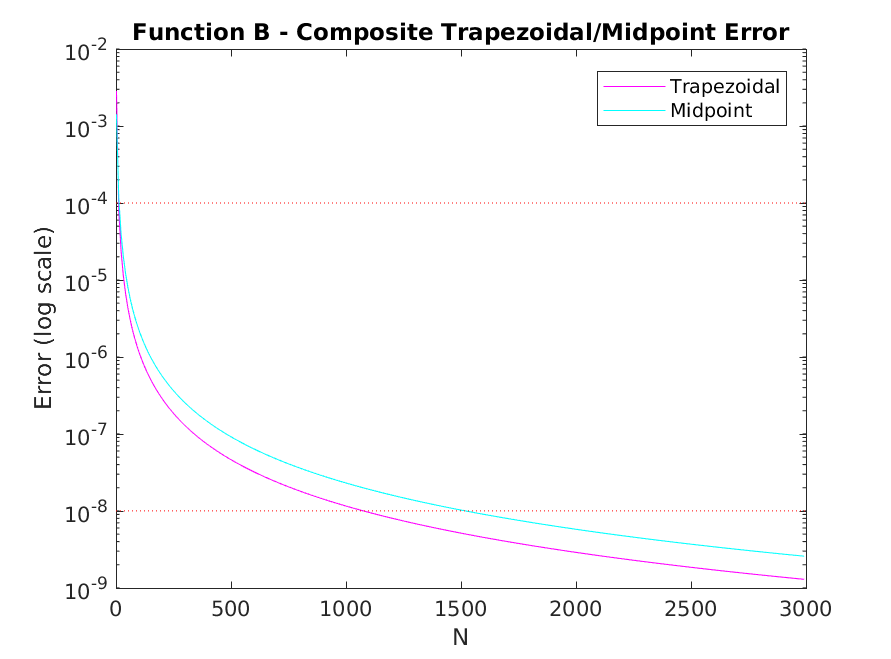
\includegraphics[width=0.7\textwidth]{../output/b_trapezoidal_midpoint.png}
	\captionof{figure}{Plot of error from Trapezoidal and Midpoint integration of Function B}
	\label{fig:b_trap_mid}
\end{center}


\subsection{Simpson's Results}\label{results:sim}

The effectiveness of Simpson's Rule as indicated by its higher order error term, discussed earlier, is clearly evident in the plot of the error for each function across the range of \textbf{n} values, seen in Figures \ref{fig:a_sim} and \ref{fig:b_sim}.

\begin{center}
	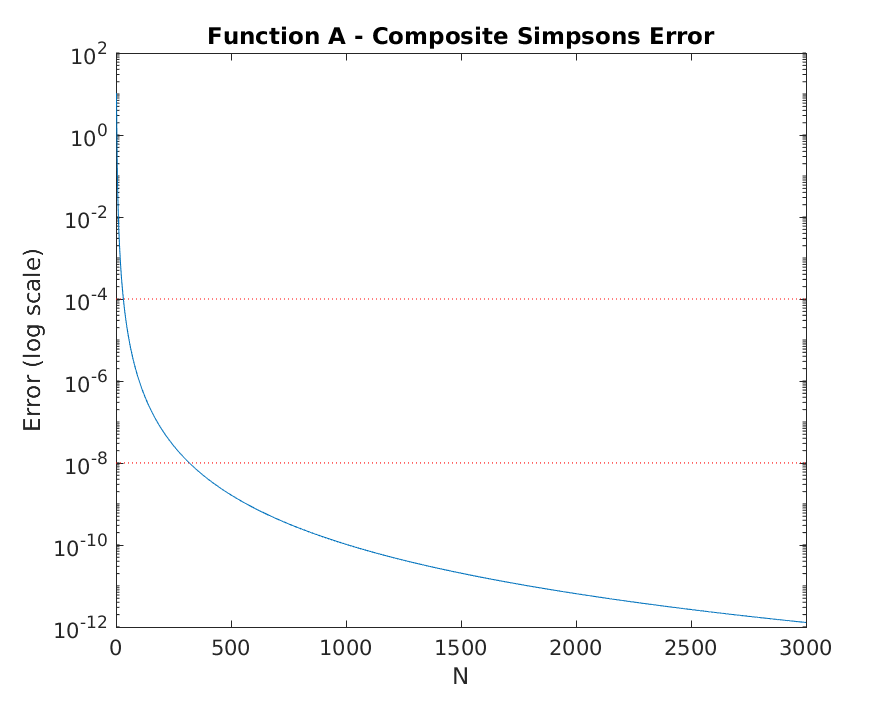
\includegraphics[width=0.7\textwidth]{../output/a_simpsons.png}
	\captionof{figure}{Plot of error from Simpson's integration of Function A}
	\label{fig:a_sim}
\end{center}

Although notably faster at reaching the tolerance levels of both $10^{-4}$ and $10^{-8}$ for Function A, it slows down as the error nears $10^{-12}$ - possibly an attribute of the function rather than Simpson's Rule. When used with Function B, Simpson's Rule reaches an error of around $10^{-15}$ in around only 1000 iterations. At this level of error, floating point precision and the limitations of the precision that MATLAB can handle\footnote{See following link on MATLAB precision limitions (general limitations of floating point representations apply) https://www.mathworks.com/help/fixedpoint/ug/limitations-on-precision.html} becomes apparent. In Figure \ref{fig:b_sim} the fluctuations causes by hitting this limit of precision can be seen between \textbf{n} values of 1000 and 3000. 
 
\begin{center}
	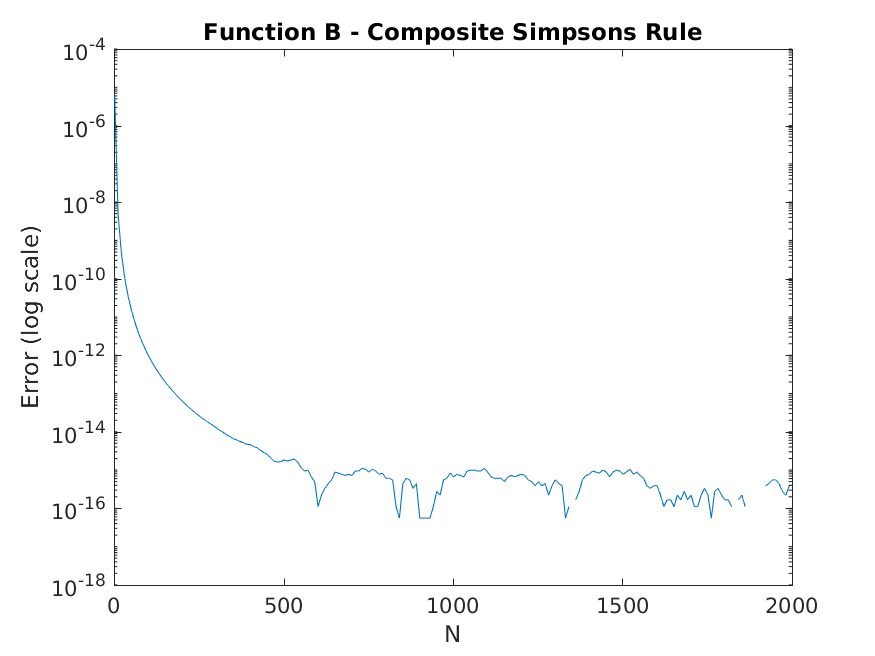
\includegraphics[width=0.7\textwidth]{../output/b_simpsons.png}
	\captionof{figure}{Plot of error from Simpson's integration of Function B}
	\label{fig:b_sim}
\end{center}



\subsection{Adaptive Simpson's Results}\label{results:adaptive}

Based on the true function plots in Figure \ref{fig:true} it is reasonable to expect that an adaptive approach may yield some benefit for Function A due to the variable nature of the function over this range, while Function B has a relatively minor and fairly consistent slope and would not be a good use case for an adaptive method.


\begin{center}
    \centering
    \begin{minipage}{0.5\textwidth}
        \centering
        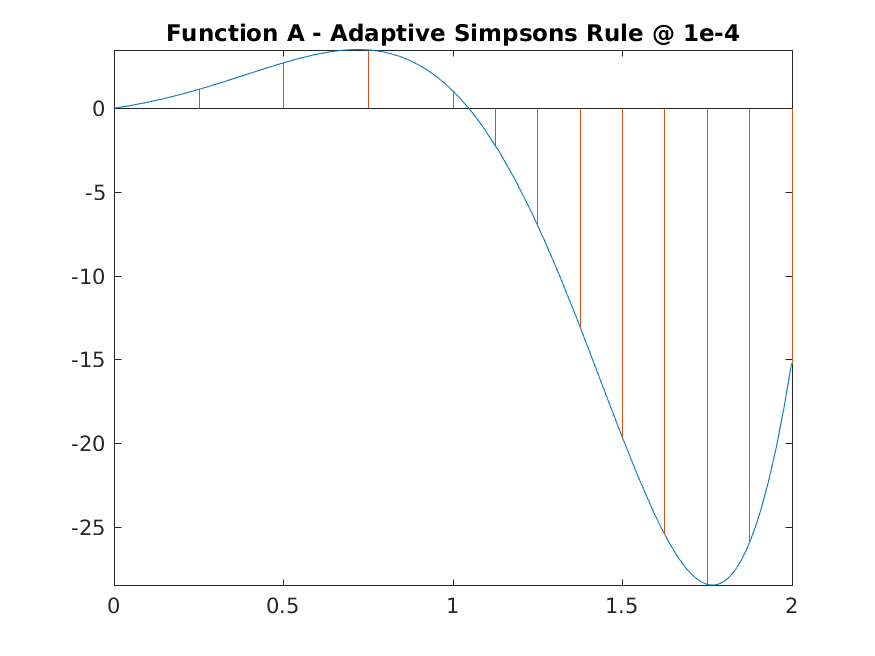
\includegraphics[width=0.99\textwidth]{../output/a_adaptive_simpsons_4.png}
    \end{minipage}\hfill
    \begin{minipage}{0.5\textwidth}
        \centering
        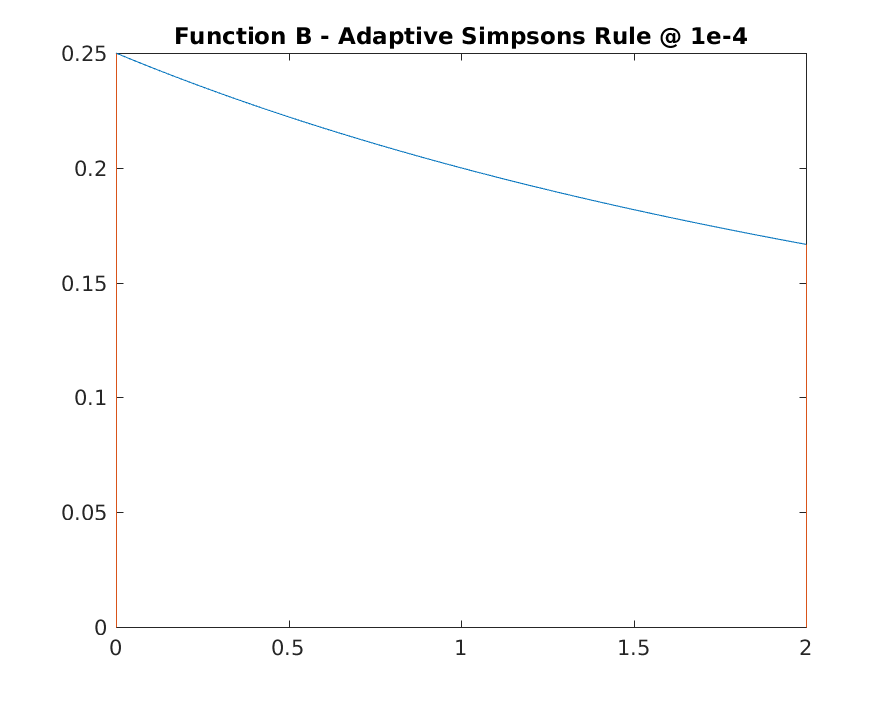
\includegraphics[width=0.99\textwidth]{../output/b_adaptive_simpsons_4.png}
    \end{minipage}
  	\captionof{figure}{Subintervals generated by adaptive Simpson's Rule for Function A and B with tolerance of $10^{-4}$}
	\label{fig:adap4}
\end{center}


Figure \ref{fig:adap4} shows the subinterval pairs generated by the application of the adaptive Simpsons's Rule with a relatively high tolerance of $10^{-4}$. Although there is some minor variation in the values of \textbf{h} for Function A, Function B required only a single subinterval pair to reach the tolerance and clearly did not need an adaptive approach. When the tolerance is reduced to $10^{-8}$, Function B still has no variance in the values of \textbf{h} over the 16 subintervals generated, seen in Figure \ref{fig:b_adap8}. Function A, however, does benefit slightly over the 278 subinterval pairs seen in Figure \ref{fig:a_adap8}. The distribution of the size of subintervals can be seen in Figure \ref{fig:a_adap8_hist}.


\begin{center}
	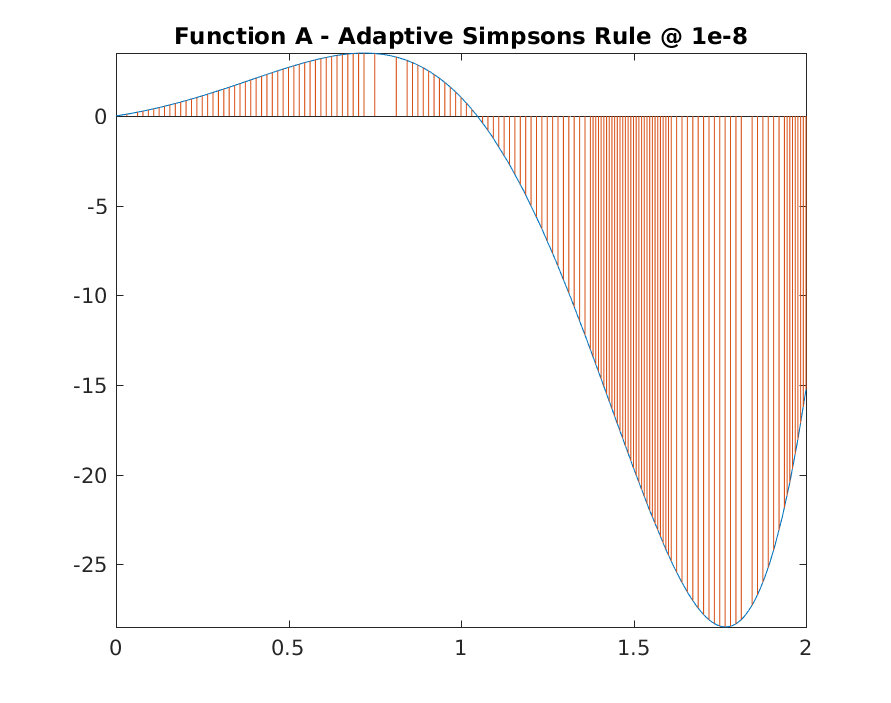
\includegraphics[width=0.7\textwidth]{../output/a_adaptive_simpsons_8.png}
	\captionof{figure}{Subintervals generated by adaptive Simpson's Rule for Function A with tolerance of $10^{-8}$}
	\label{fig:a_adap8}
\end{center}

\begin{center}
	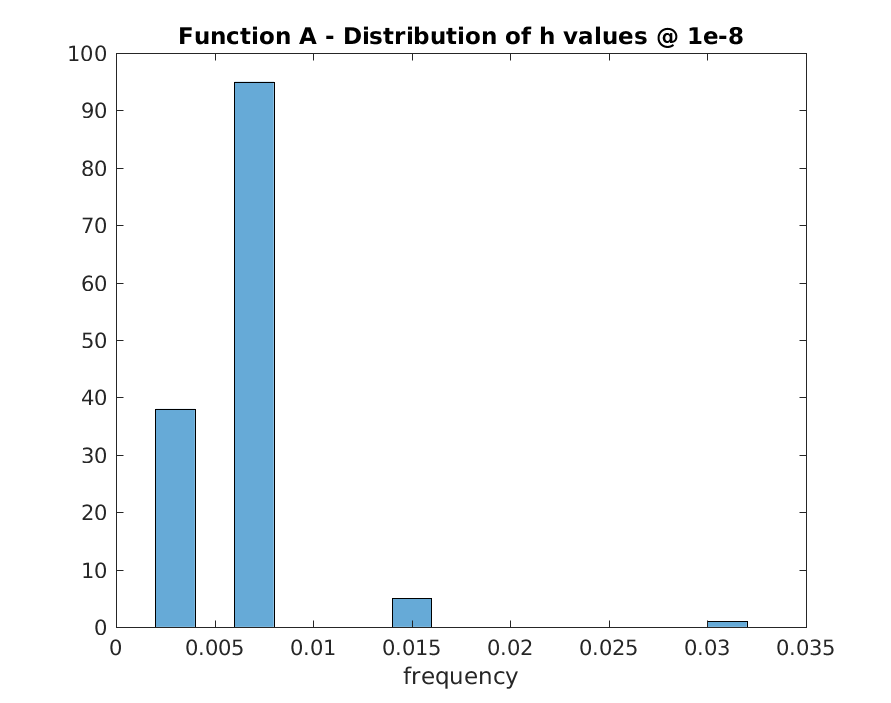
\includegraphics[width=0.7\textwidth]{../output/a_adaptive_simpsons_8_hist.png}
	\captionof{figure}{Distribution of the size of subintervals generated from adaptive Simpson's for Function A}
	\label{fig:a_adap8_hist}
\end{center}


\begin{center}
	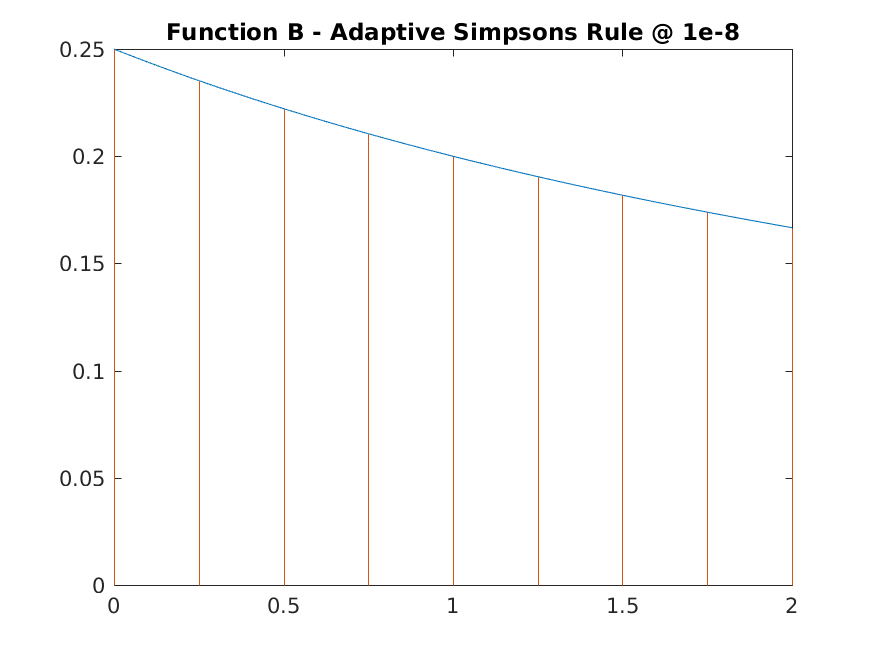
\includegraphics[width=0.65\textwidth]{../output/b_adaptive_simpsons_8.png}
	\captionof{figure}{Subintervals generated by adaptive Simpson's Rule for Function B with tolerance of $10^{-8}$}
	\label{fig:b_adap8}
\end{center}


If the range over which the integral was taken is expanded, as seen in Figure \ref{fig:expanded}, an adaptive approach becomes much more useful. When expanded with a lower bound of -2 and an upper bound of 3, Function A has a substantial portion of the range between -2 and 1 where the integral will be close to zero. The adaptive approach would reduce \textbf{h} over this range, and then between 1 and 3,  where there is significant variation in the function and a larger relative integral, the value of \textbf{h} would increase as needed. Similarly, when Function B is expanded to -3.9 and 2, the integral between -3.9 and -3 is much larger relative to the integral between -3 and 2. In this case, the adaptive approach to integration would again prove useful\footnote{Function B has a vertical asymptote at -4 which introduces a complication when calculating the integral as it is technically infinite at -4. A practical approach to calculating this integral would be to split the calculation into one part up to just before -4 and another part start just after -4}.

\begin{center}
    \centering
    \begin{minipage}{0.5\textwidth}
        \centering
        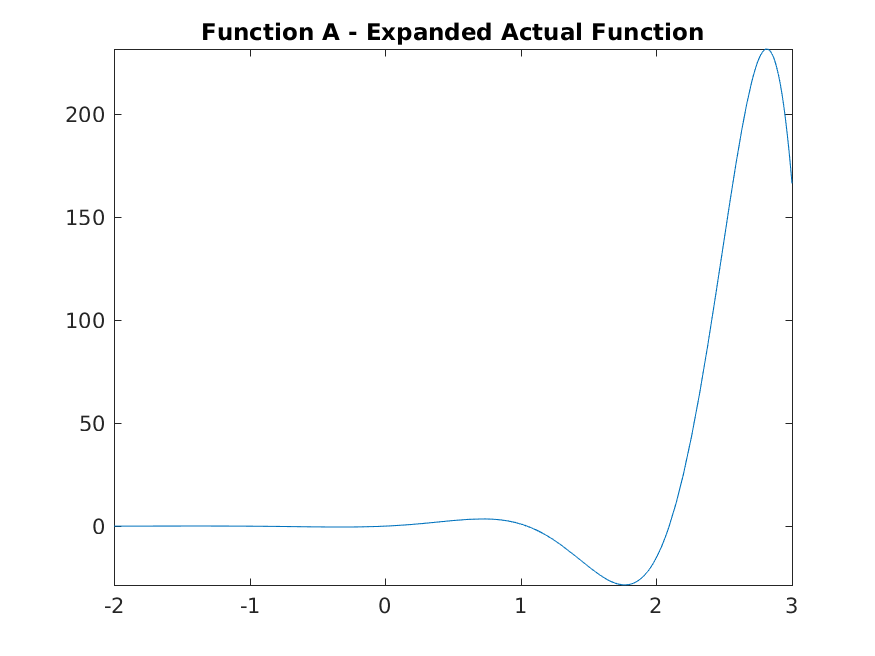
\includegraphics[width=0.99\textwidth]{../output/a_expanded_actual.png}
    \end{minipage}\hfill
    \begin{minipage}{0.5\textwidth}
        \centering
        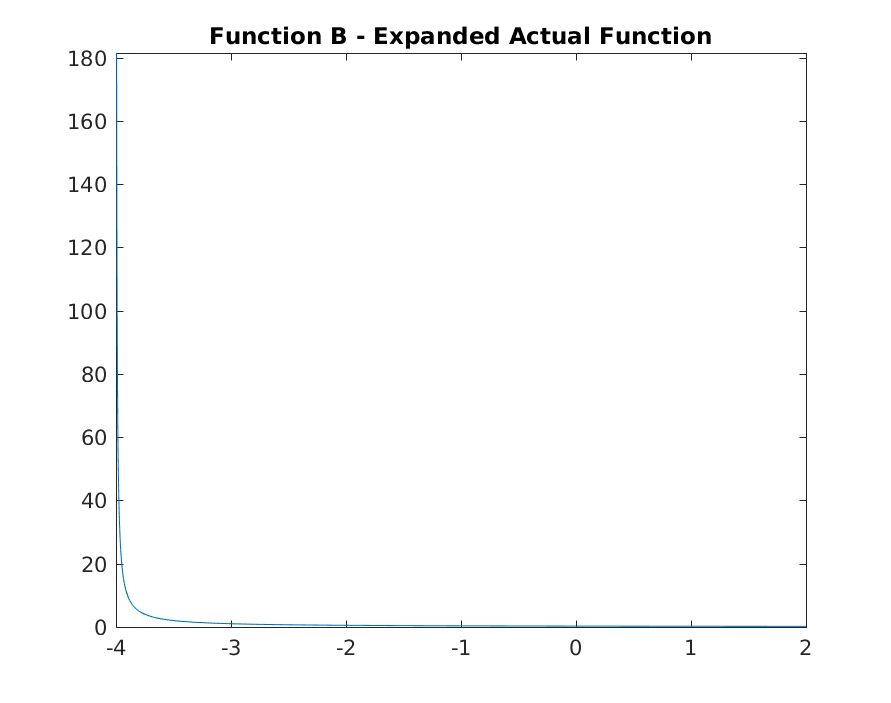
\includegraphics[width=0.99\textwidth]{../output/b_expanded_actual.png}
    \end{minipage}
  	\captionof{figure}{True plots of Function A and B over expanded range}
	\label{fig:expanded}

\end{center}



\newpage

\bibliography{report}


\end{document}
